\documentclass{beamer}
\usepackage{graphicx} % For including images
\usepackage{amsmath}  % For mathematical equations
\usepackage{amssymb}  % For mathematical symbols
\usepackage{hyperref} % For hyperlinks
\usepackage{booktabs} % For better table formatting
\usepackage{subcaption} % For subfigures
\usepackage{media9}



\usetheme{Madrid} % Choose a theme (e.g., Madrid, Berlin, etc.)
\setbeamertemplate{footline}{}

\title{Statistical Analysis of Deepfake Images and Videos in Smart City Applications}
\author{ANAND M K}
\institute{242CS008}
\date{}

\begin{document}

\begin{frame}
    \titlepage
\end{frame}

\begin{frame}{Introduction}
    \begin{itemize}
        \item Deepfake technology uses advanced machine learning algorithms (e.g., GANs) to create synthetic media.
        \item Risks in smart cities: Surveillance, traffic monitoring, and public safety rely on authentic media.
        \item Focus: Statistical analysis of deepfake datasets to identify patterns and anomalies.
    \end{itemize}
\end{frame}

\begin{frame}{Datasets Used}
    \begin{itemize}
        \item \textbf{FaceForensics}: Real and manipulated videos.
        \item \textbf{OpenForensics}: Real and synthetic images.
        \item \textbf{UADFV}: Real and deepfake videos.
    \end{itemize}
    \begin{figure}
        \centering
        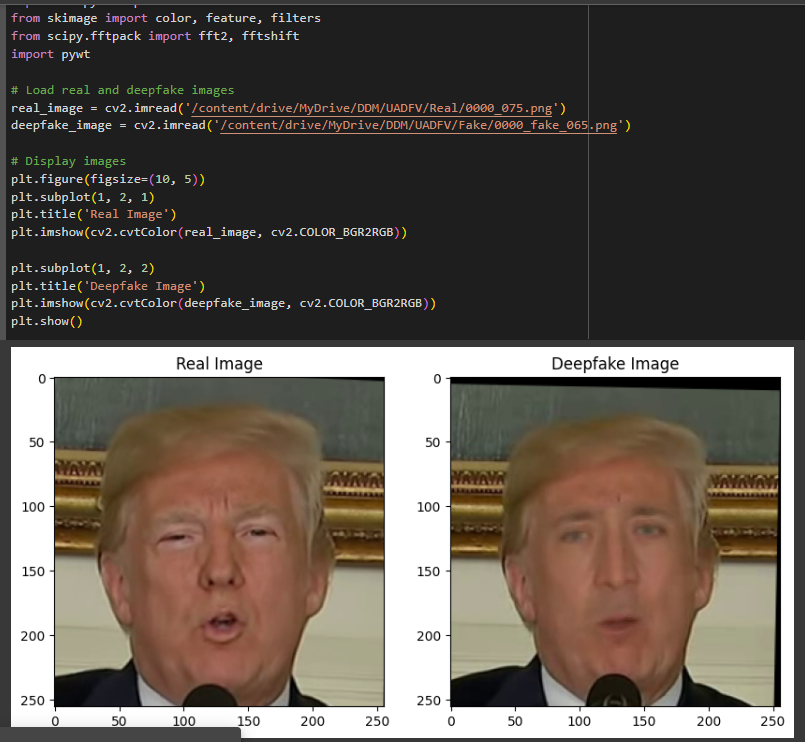
\includegraphics[width=0.5\textwidth]{dataset_screenshot.png} % Replace with screenshot of dataset loading
        \caption{Screenshot: Loading datasets in Colab.}
    \end{figure}
\end{frame}

\begin{frame}{Descriptive Statistics}
    \begin{itemize}
        \item \textbf{Mean, Median, Mode}: Central tendency of pixel intensities.
        \item \textbf{Variance, Standard Deviation}: Spread of pixel values.
        \item \textbf{Histograms}: Distribution of pixel intensities.
        \item \textbf{Correlation}: Relationship between pixel values.
        \item \textbf{Temporal Statistics}: Frame-by-frame changes in videos.
    \end{itemize}
    \begin{figure}
        \centering
        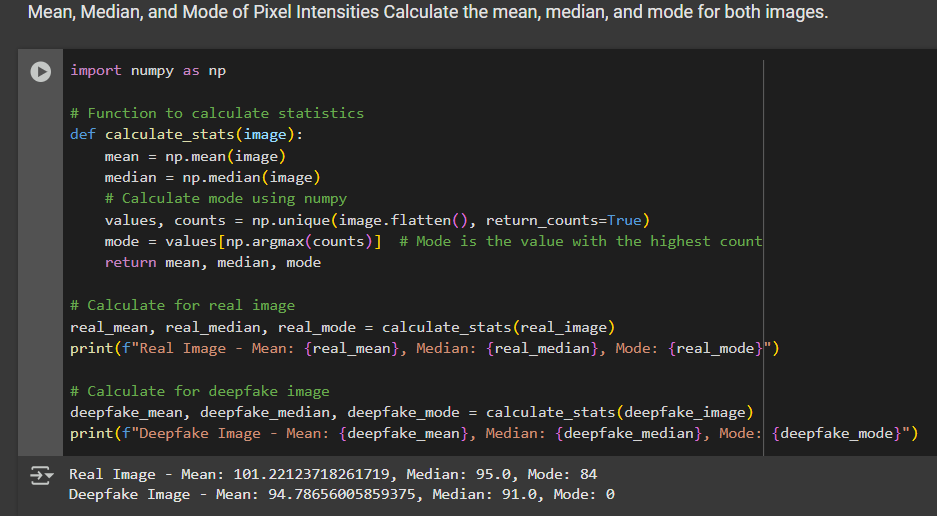
\includegraphics[width=0.7\textwidth]{mean.png} % Replace with screenshot of code execution
        \caption{Screenshot: Calculate the mean, median, and mode.}
    \end{figure}
\end{frame}

\begin{frame}{Descriptive Statistics}
    \begin{figure}
        \centering
        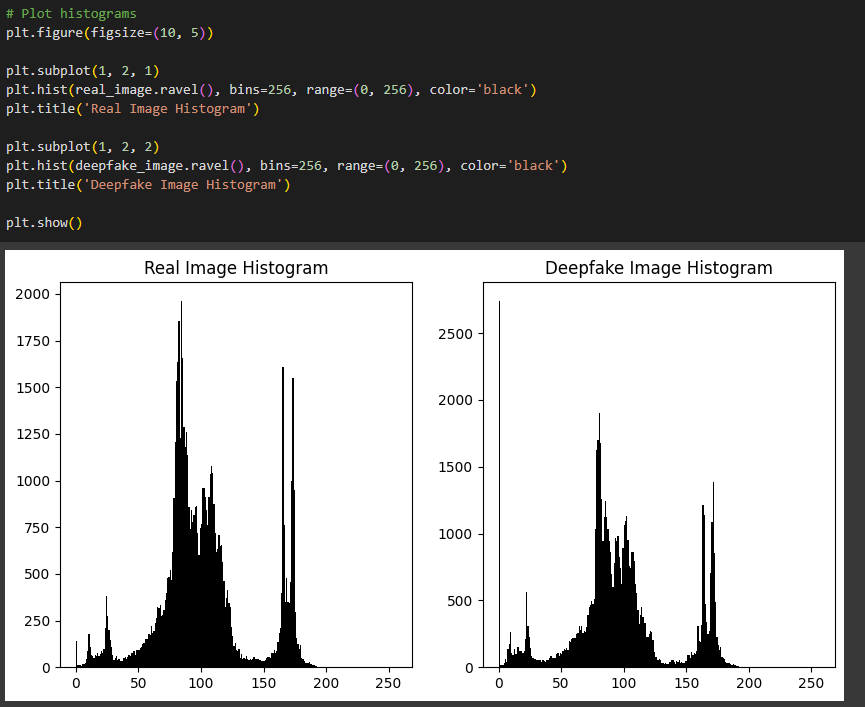
\includegraphics[width=0.7\textwidth]{histo.png} % Replace with screenshot of code execution
        \caption{Screenshot: Plot histograms.}
    \end{figure}
\end{frame}

\begin{frame}{Descriptive Statistics}
    \begin{figure}
        \centering
        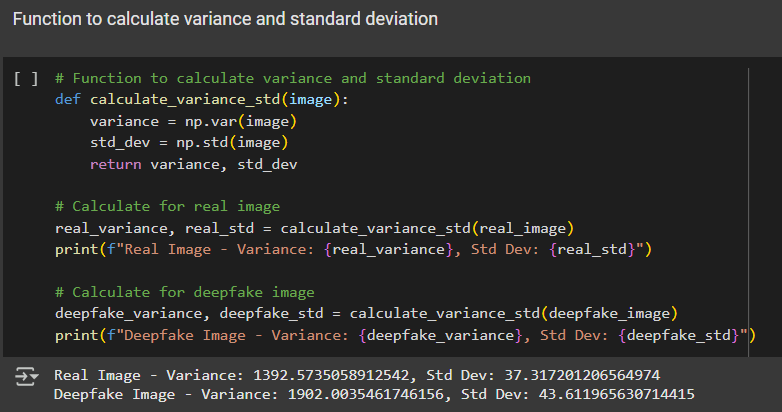
\includegraphics[width=0.8\textwidth]{std.png} % Replace with screenshot of code execution
        \caption{Screenshot: Calculate variance and standard deviation.}
    \end{figure}

\end{frame}


\begin{frame}{Feature Extraction}
    \begin{itemize}
        \item \textbf{Canny Edge Detection}: Detects edges in images.
        \item \textbf{Haralick Features}: Texture analysis using GLCM.
        \item \textbf{Sobel Edge Detection}: Gradient-based edge detection.
        \item \textbf{Local Binary Patterns (LBP)}: Texture descriptor.
        \item \textbf{Fourier Transform}: Frequency domain analysis.
        \item \textbf{Wavelet Transform}: Multi-resolution analysis.
        \item \textbf{Average Frame Difference}: Temporal analysis of videos.
    \end{itemize}
    
\end{frame}

\begin{frame}{Feature Extraction}
 	\begin{figure}
    \end{figure}
\end{frame}
\begin{frame}{Feature Extraction}
 	\begin{figure}
    \end{figure}
\end{frame}
\begin{frame}{Feature Extraction}
 	\begin{figure}
    \end{figure}
\end{frame}

\begin{frame}{Statistical Modeling}
    \begin{itemize}
        \item \textbf{Gaussian Mixture Models (GMM)}: Models pixel intensity distributions.
        \item \textbf{Hidden Markov Models (HMM)}: Models temporal sequences in videos.
    \end{itemize}
    \begin{figure}
        \centering
        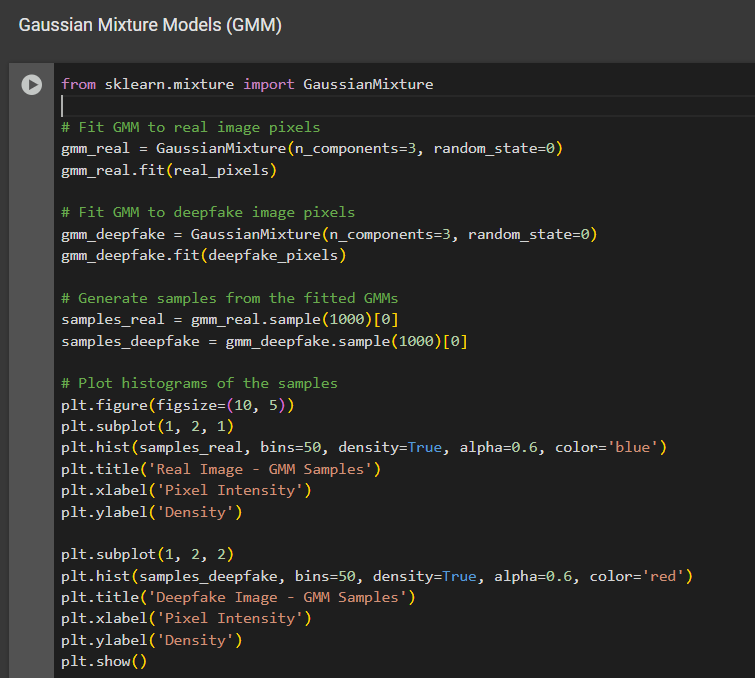
\includegraphics[width=0.5\textwidth]{gmm.png} % Replace with screenshot of code execution
        \caption{Screenshot: GMM code execution.}
    \end{figure}
\end{frame} 

\begin{frame}{Statistical Modeling}
    \begin{figure}
        \centering
        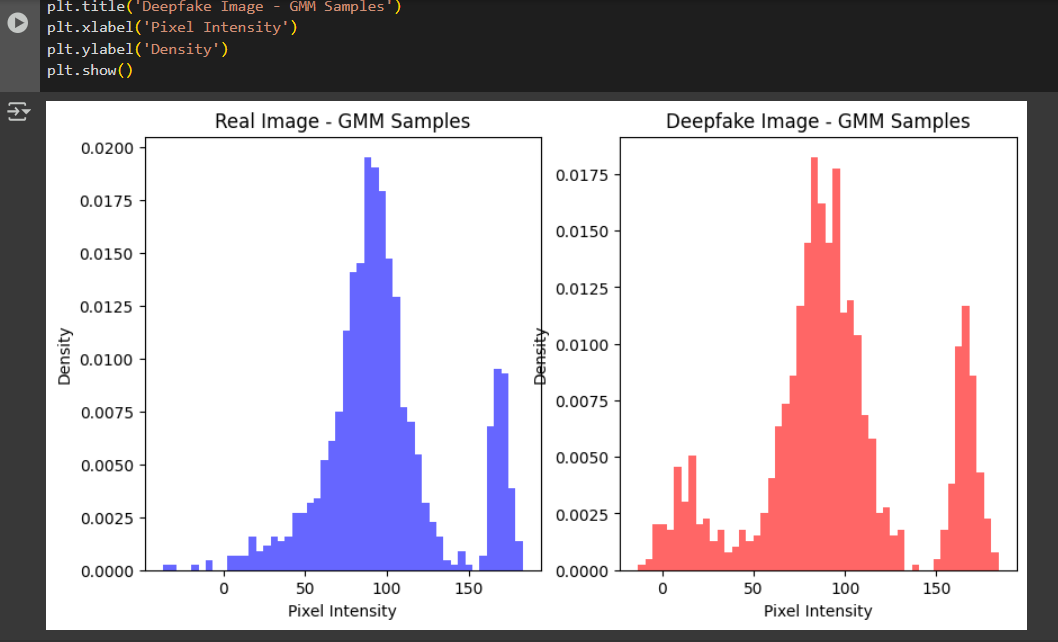
\includegraphics[width=0.8\textwidth]{gmm2.png} % Replace with screenshot of code execution
        \caption{Screenshot: GMM code execution.}
    \end{figure}
\end{frame} 

\begin{frame}{Statistical Modeling}
    \begin{figure}
        \centering
        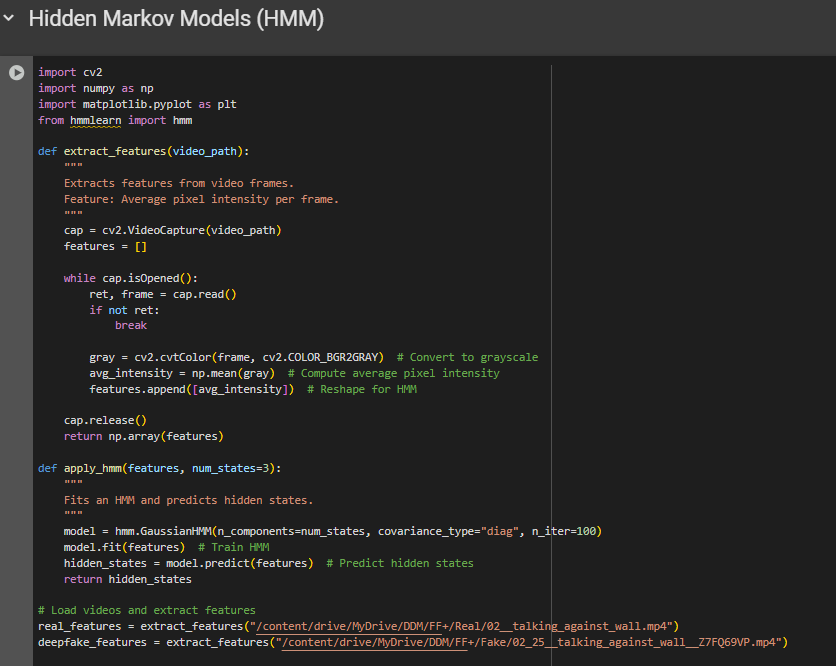
\includegraphics[width=0.8\textwidth]{hmm1.png} % Replace with screenshot of code execution
        \caption{Screenshot: HMM code execution.}
    \end{figure}
\end{frame} 

\begin{frame}{Statistical Modeling}
    \begin{figure}
        \centering
        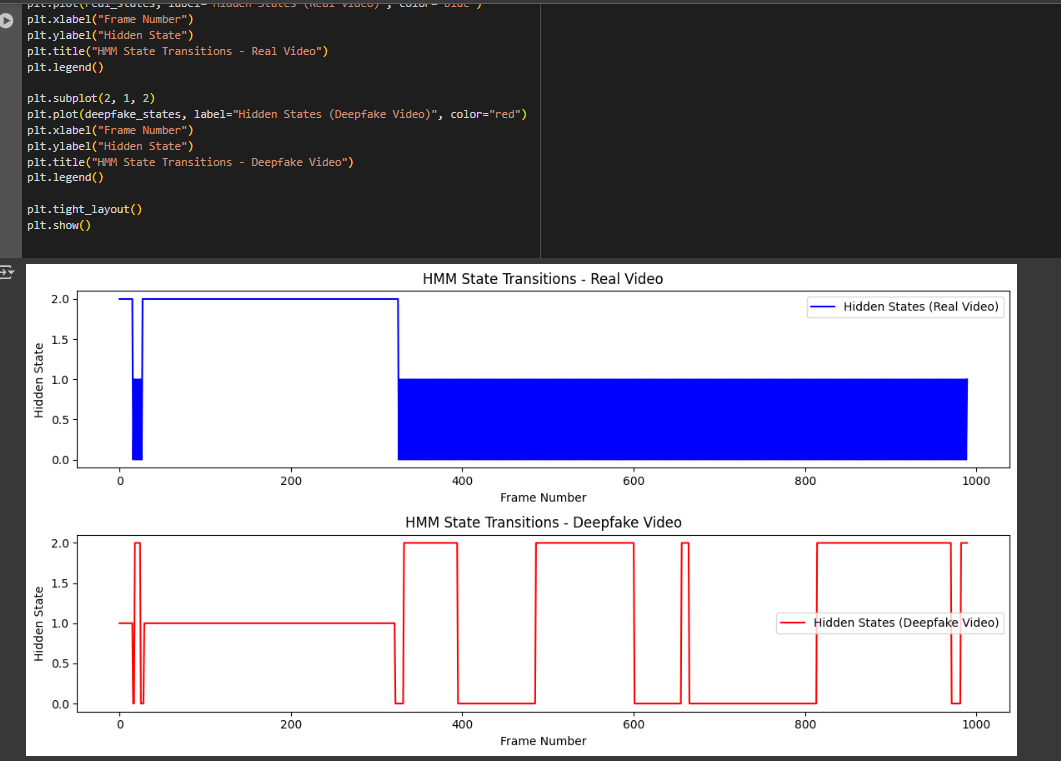
\includegraphics[width=0.8\textwidth]{hmm2.png} % Replace with screenshot of code execution
        \caption{Screenshot: HMM code execution.}
    \end{figure}
\end{frame} 

\begin{frame}{Statistical Tools}
    \begin{itemize}
        \item \textbf{OpenCV}: Image and video processing.
        \item \textbf{Scikit-Image}: Texture and edge analysis.
        \item \textbf{Matlab}: Fourier and fractal analysis.
        \item \textbf{PyTorch/TensorFlow}: Deep learning-based analysis.
        \item \textbf{NumPy/SciPy}: Basic statistical operations.
    \end{itemize}
\end{frame}

\begin{frame}{Conclusion}
    \begin{itemize}
        \item Statistical methods (descriptive statistics, feature extraction, modeling) effectively differentiate real and deepfake media.
        \item Tools like OpenCV, Scikit-Learn, and HMMLearn were instrumental in implementation.
        \item Future work: Integrate deep learning models and explore larger datasets.
        \item Overall, statistical analysis provides a strong foundation for deepfake detection.
    \end{itemize}
\end{frame}


\end{document}